% !TeX program = xelatex
\documentclass[UTF8,fontset=none,10pt,a4paper,twocolumn]{ctexart}

\usepackage[margin=1.65cm,top=1.55cm,bottom=1.45cm,columnsep=0.68cm]{geometry}
\usepackage{amsmath,amssymb}
\usepackage{booktabs}
\usepackage{tabularx}
\usepackage{array}
\usepackage{enumitem}
\usepackage{fancyhdr}
\usepackage{titlesec}
\usepackage{xcolor}
\usepackage{graphicx}
\usepackage{tikz}
\usepackage{xurl}
\usepackage{hyperref}
\usepackage{iftex}
\usetikzlibrary{arrows.meta,positioning,calc,fit}

\ifPDFTeX
  \PackageError{paper}{This document requires XeLaTeX}{Set the Overleaf compiler to XeLaTeX.}
\fi
\ifXeTeX
  \IfFontExistsTF{FandolSong-Regular}{
    \setCJKmainfont{FandolSong-Regular}
    \setCJKsansfont{FandolHei-Regular}
    \setCJKmonofont{FandolFang-Regular}
  }{
    \IfFontExistsTF{Noto Serif CJK SC}{
      \setCJKmainfont{Noto Serif CJK SC}
      \setCJKsansfont{Noto Sans CJK SC}
      \setCJKmonofont{Noto Sans Mono CJK SC}
    }{
      \setCJKmainfont{SimSun}
    }
  }
\fi

\setlength{\parindent}{2em}
\setlength{\parskip}{0pt}
\linespread{1.04}
\pagestyle{fancy}
\fancyhf{}
\fancyhead[L]{数据挖掘课程项目}
\fancyhead[R]{LLM 空间推理行为挖掘}
\fancyfoot[C]{\thepage}
\renewcommand{\headrulewidth}{0.35pt}

\titleformat{\section}{\large\bfseries}{\thesection}{0.55em}{}
\titleformat{\subsection}{\normalsize\bfseries}{\thesubsection}{0.45em}{}
\titleformat{\subsubsection}{\normalsize\bfseries}{\thesubsubsection}{0.45em}{}
\titlespacing*{\section}{0pt}{0.8em}{0.35em}
\titlespacing*{\subsection}{0pt}{0.55em}{0.25em}
\setlist[itemize]{leftmargin=1.35em,itemsep=0pt,topsep=2pt}
\setlist[enumerate]{leftmargin=1.55em,itemsep=0pt,topsep=2pt}
\hypersetup{hidelinks}
\urlstyle{tt}
\sloppy

\newcolumntype{Y}{>{\raggedright\arraybackslash}X}
\newcommand{\code}[1]{\texttt{\detokenize{#1}}}
\newcommand{\mcode}[1]{\text{\ttfamily\detokenize{#1}}}
\definecolor{dmblue}{HTML}{2F5E8E}
\definecolor{dmgreen}{HTML}{3F7F5F}
\definecolor{dmorange}{HTML}{C47A2C}
\definecolor{dmgray}{HTML}{F2F4F7}
\tikzset{
  dmblock/.style={draw=dmblue!75, fill=dmblue!7, rounded corners=2pt,
    align=center, font=\scriptsize, inner sep=4pt, minimum height=1.9em},
  dmblockgreen/.style={draw=dmgreen!80, fill=dmgreen!8, rounded corners=2pt,
    align=center, font=\scriptsize, inner sep=4pt, minimum height=1.9em},
  dmblockorange/.style={draw=dmorange!80, fill=dmorange!10, rounded corners=2pt,
    align=center, font=\scriptsize, inner sep=4pt, minimum height=1.9em},
  dmarrow/.style={-{Latex[length=2mm]}, line width=0.45pt, draw=black!65},
  dmnote/.style={font=\scriptsize, align=center, text=black!78}
}

\begin{document}

\twocolumn[
\begin{@twocolumnfalse}
\begin{center}
{\Large\bfseries 大语言模型在轮椅转弯空间推理中的行为挖掘研究\par}
\vspace{0.25em}
{\normalsize Behavior Mining of Large Language Models in Wheelchair Turning Spatial Reasoning\par}
\vspace{0.45em}
{\small 单屹 \quad 张驰 \quad 徐敬研 \quad 傅玉 \quad 董梓苏 \quad 黄鸣辉\par}
\end{center}
\vspace{0.25em}
\noindent\textbf{摘要}\quad
本文研究大语言模型在轮椅转弯空间推理中的行为稳定性、噪声敏感性与失效模式。我们将“电动轮椅能否在楼梯转角处完成 $90^\circ$ 转弯”建模为一个受控文本推理任务，把场景表示为通道净宽、平台进深、轮椅宽度、轮椅长度和最小转弯半径等几何变量，并围绕描述层级、无关扰动和场景生成策略构造 Prompt 实验矩阵。与只报告单次准确率不同，本文把模型回复视为可挖掘的行为数据：每条记录同时保留 Prompt 条件、模型、重复编号、原始回复、解析判断和失败类别，从而分析模型何时依赖常识直觉，何时尝试形式化建模，以及哪些非因果线索会诱发判断翻转。正式实验选取 5 组代表性 Prompt 来源，每组 300 条，共 1500 条样本，并通过 DF/OpenAI-compatible 网关调用 12 个模型、每个样本重复采样 3 次，形成 $1500\times 12\times 3=54{,}000$ 条原始模型行为记录。本文给出任务定义、相关工作、Prompt 矩阵、多模型采集协议、行为特征接口和挖掘分析框架，作为完整实验数据分析与结果解释的基础。
\par\vspace{0.3em}
\noindent\textbf{关键词}\quad 大语言模型；空间推理；行为挖掘；轮椅转弯；扰动敏感性；失效模式
\vspace{0.85em}
\end{@twocolumnfalse}
]

\section{研究任务与数据来源}

本项目关注的问题是：当大语言模型面对一个关于“电动轮椅能否在楼梯转角处完成 $90^\circ$ 转弯”的空间推理问题时，它的最终判断是否稳定、是否受表达层级和无关扰动影响，以及不同模型之间是否呈现可挖掘的失效模式。这里的核心对象不是单个几何题答案，而是模型在受控 Prompt 条件下产生的行为记录。

上游 Prompt 生成部分已经把一个空间场景表示为五元组
\begin{equation}
\mathbf{x}=(W,D,w,L,R),
\end{equation}
其中 $W$ 是楼梯通道净宽，$D$ 是平台有效进深，$w$ 和 $L$ 分别表示轮椅宽度与长度，$R$ 是厂家或题干给出的保守最小转弯半径，单位均为厘米。为了给后续评价提供一致参照，数据集中定义几何余量
\begin{equation}
\kappa(\mathbf{x})=\min(W-w,\ D-R).
\label{eq:clearance-margin}
\end{equation}
若 $\kappa\geq 3$，参考标签记为 \code{can_pass}；否则记为 \code{cannot_pass}。这些标签不会暴露给模型，只在后续特征构建和准确性分析时使用。

\begin{figure}[t]
\centering
\begin{tikzpicture}[scale=0.78, every node/.style={font=\scriptsize}]
  \fill[dmgray] (-0.25,-0.25) rectangle (5.15,3.65);
  \fill[white] (0,0) rectangle (4.8,1.15);
  \fill[white] (3.65,0) rectangle (4.8,3.4);
  \draw[black!55, line width=0.45pt] (0,1.15) -- (3.65,1.15) -- (3.65,3.4);
  \draw[black!55, line width=0.45pt] (0,0) -- (4.8,0) -- (4.8,3.4);
  \draw[dmorange, dashed, line width=0.7pt] (2.72,1.15) arc[start angle=180,end angle=90,radius=0.93];
  \node[dmnote, dmorange] at (3.15,1.78) {$R$};
  \draw[fill=dmgreen!18, draw=dmgreen!80, rounded corners=1.5pt, rotate around={8:(2.65,0.55)}]
    (2.22,0.26) rectangle (3.08,0.84);
  \draw[<->, black!65] (2.22,0.08) -- (3.08,0.08)
    node[midway,below] {$L$};
  \draw[<->, black!65] (3.25,0.26) -- (3.25,0.84)
    node[midway,right] {$w$};
  \draw[<->, black!65] (-0.1,0) -- (-0.1,1.15)
    node[midway,left] {$W$};
  \draw[<->, black!65] (3.65,3.55) -- (4.8,3.55)
    node[midway,above] {$D$};
  \node[dmnote] at (2.0,1.42) {楼梯转角平台};
  \node[dmnote] at (4.25,2.55) {转向通道};
\end{tikzpicture}
\caption{轮椅转弯空间推理任务的抽象几何示意。实验并不追求真实工程仿真，而是固定 $W,D,w,L,R$ 等关键变量，用受控 Prompt 观察模型如何利用或误用这些空间信息。}
\label{fig:task-geometry}
\end{figure}


每条 Prompt 可以抽象为
\begin{equation}
p=f(\mathbf{x},\ell,n,g),
\end{equation}
其中 $\ell\in\{\mathrm{L1},\mathrm{L2},\mathrm{L3}\}$ 表示描述层级，$n$ 表示扰动条件，$g$ 表示场景生成策略。模型 $m$ 在第 $r$ 次重复采样中的回复记为 $a_{m,r}(p)$。这一记号使后续分析能够直接按策略、层级、扰动、模型和重复编号进行分组。

\section{Prompt 实验矩阵}

\subsection{层级与扰动变量}

同一个空间场景被写成三个描述层级。L1 更接近日常语言，只给出转角紧凑、轮椅较宽等模糊描述；L2 给出 $W,D,w,L,R$ 等具体数值，观察模型是否会进行参数比较；L3 将场景表述为 L 形通道、矩形刚体和旋转包络，用来测试形式化描述是否诱发新的概念混淆。三个层级的问题目标和最终回答格式保持一致。

扰动条件用于检验模型是否会被非因果信息牵引。扰动文本不改变 $\mathbf{x}$、$\kappa$ 或参考标签，只改变题干中的背景细节，例如墙面材质、环境噪声、光照状态或旁观者催促。若模型在相同空间参数下因为这些信息改变最终判断，就说明其空间推理链条存在不稳定性。

\begin{table}[t]
\centering
\caption{扰动条件与预期作用}
\label{tab:noise}
\small
\begin{tabularx}{\columnwidth}{p{0.36\columnwidth}Y}
\toprule
扰动标签 & 设计目的 \\
\midrule
\code{none} & 纯几何描述，作为基线条件。\\
\code{material_color} & 加入扶手颜色、墙面材质，测试视觉细节牵引。\\
\code{ambient_noise} & 加入现场噪声，测试环境语义干扰。\\
\code{lighting} & 加入光照与地面状态，测试风险联想是否覆盖几何判断。\\
\code{emotional_pressure} & 加入催促和紧张语境，测试情绪压力是否诱发保守偏置。\\
\bottomrule
\end{tabularx}
\end{table}

\subsection{场景生成策略}

完整 Prompt 候选池包含一个基线策略和多组实验设计型扩展策略。每种策略产生 20 个空间场景，并与 3 个描述层级、5 类扰动做笛卡尔积，因此单个策略对应
\begin{equation}
20 \text{ scenarios}\times 3 \text{ levels}\times 5 \text{ noises}=300
\end{equation}
条 Prompt。策略字段必须在合并后保留，因为不同策略文件中可能存在相同的 \code{prompt_id}；若只使用文件内编号，断点续跑和分组分析都会产生歧义。

\begin{figure*}[t]
\centering
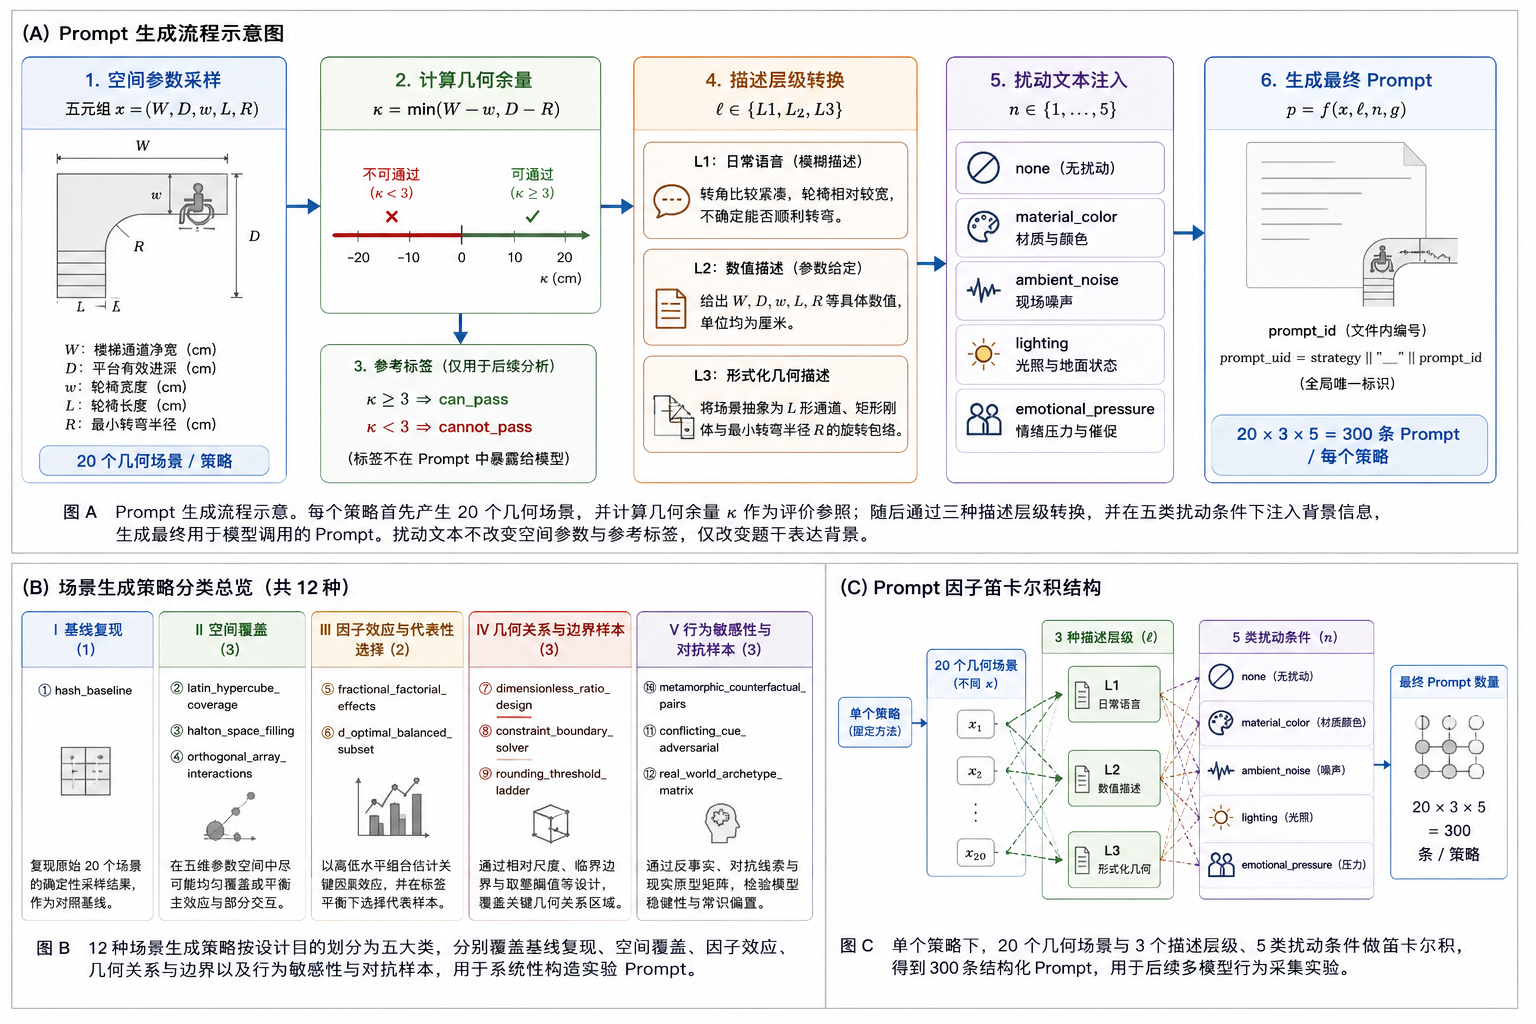
\includegraphics[width=0.92\textwidth,height=0.56\textheight,keepaspectratio]{figures/prompts_gen.png}
\caption{上游 Prompt 生成流程示意。该流程负责从轮椅转弯空间参数、描述层级、扰动条件和场景生成策略出发，构造可复现的 Prompt 候选池；本文后续的多模型 API 实验不重写该生成逻辑，而是复用其输出并进一步采集模型行为数据。}
\label{fig:prompts-gen}
\end{figure*}


\begin{figure*}[t]
\centering
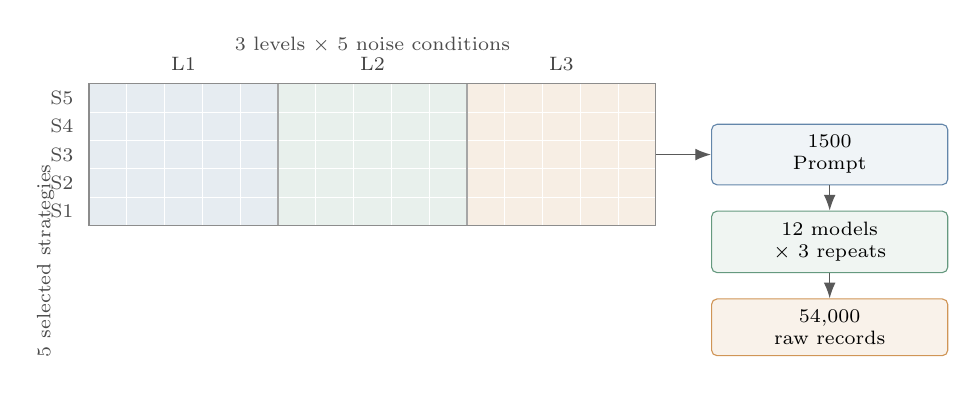
\begin{tikzpicture}[x=0.48cm,y=0.36cm, every node/.style={font=\scriptsize}]
  \foreach \y/\lab in {0/S1,1/S2,2/S3,3/S4,4/S5} {
    \foreach \x in {0,...,14} {
      \pgfmathtruncatemacro{\grp}{int(\x/5)}
      \ifnum\grp=0
        \fill[dmblue!12] (\x,\y) rectangle ++(1,1);
      \else\ifnum\grp=1
        \fill[dmgreen!12] (\x,\y) rectangle ++(1,1);
      \else
        \fill[dmorange!13] (\x,\y) rectangle ++(1,1);
      \fi\fi
      \draw[white, line width=0.35pt] (\x,\y) rectangle ++(1,1);
    }
    \node[anchor=east, text=black!70] at (-0.15,\y+0.5) {\lab};
  }
  \draw[black!45] (0,0) rectangle (15,5);
  \foreach \x/\lab in {2.5/L1,7.5/L2,12.5/L3} {
    \node[anchor=south, text=black!75] at (\x,5.12) {\lab};
  }
  \foreach \x in {5,10} {
    \draw[black!35, line width=0.6pt] (\x,0) -- (\x,5);
  }
  \node[anchor=east, rotate=90, text=black!70] at (-1.15,2.5) {5 selected strategies};
  \node[anchor=south, text=black!70] at (7.5,5.75) {3 levels $\times$ 5 noise conditions};
  \coordinate (gridright) at (15,2.5);
  \node[dmblock, right=0.7cm of gridright, minimum width=3.0cm] (p) {1500\\Prompt};
  \node[dmblockgreen, below=0.32cm of p, minimum width=3.0cm] (r) {12 models\\$\times$ 3 repeats};
  \node[dmblockorange, below=0.32cm of r, minimum width=3.0cm] (o) {54,000\\raw records};
  \draw[dmarrow] (15,2.5) -- (p.west);
  \draw[dmarrow] (p) -- (r);
  \draw[dmarrow] (r) -- (o);
\end{tikzpicture}
\caption{实验矩阵从 Prompt 控制变量扩展到模型行为记录。左侧每个小格表示一个策略、层级和扰动组合下的场景集合；右侧展示正式采集时的模型与重复采样扩展关系。}
\label{fig:experiment-tensor}
\end{figure*}


\begin{table*}[t]
\centering
\caption{上游 Prompt 场景生成策略总览}
\label{tab:strategies}
\small
\begin{tabularx}{0.96\textwidth}{p{0.27\textwidth}p{0.20\textwidth}Y}
\toprule
策略 & 方法类别 & 实验目的 \\
\midrule
\path{hash_baseline} & 哈希基线 & 复现原始 20 个场景的确定性采样结果，作为扩展策略的对照。\\
\path{latin_hypercube_coverage} & 拉丁超立方 & 均匀覆盖五个几何变量的取值区间。\\
\path{halton_space_filling} & 低差异序列 & 生成确定性但非规则的空间填充样本。\\
\path{orthogonal_array_interactions} & 正交表 & 覆盖主效应与部分二阶交互。\\
\path{fractional_factorial_effects} & 分数因子设计 & 以高低水平组合估计关键尺寸因素的方向性效应。\\
\path{d_optimal_balanced_subset} & 候选池最优子集 & 在标签平衡约束下选择代表性样本。\\
\path{dimensionless_ratio_design} & 无量纲比例 & 通过 $W/w$、$D/R$、$R/L$ 等比例检验模型是否理解相对尺度。\\
\path{metamorphic_counterfactual_pairs} & 反事实配对 & 每两条只改变一个关键参数，检验模型判断单调性。\\
\path{constraint_boundary_solver} & 边界约束求解 & 反向生成靠近阈值的临界场景。\\
\path{conflicting_cue_adversarial} & 对抗线索 & 构造宽度和转弯半径互相冲突的样本。\\
\path{real_world_archetype_matrix} & 现实原型矩阵 & 按旧住宅楼、教学楼、医院、办公楼等原型组织尺寸。\\
\path{rounding_threshold_ladder} & 取整阈值阶梯 & 围绕常见整数尺寸测试取整和常识锚定偏差。\\
\bottomrule
\end{tabularx}
\end{table*}

\section{API 调用与模型行为数据采集}

\subsection{实验样本范围}

本轮 API 实验不使用全部候选池，而是选取 5 组代表性 Prompt 来源：\path{data/prompts.csv} 作为 baseline，加上当前重点策略 \path{real_world_archetype_matrix}、\path{halton_space_filling}、\path{dimensionless_ratio_design} 和 \path{constraint_boundary_solver}。每组 300 条，共 1500 条 Prompt。这样的分层主样本同时覆盖原始基线、现实原型、空间填充、比例表达和边界临界样本，能够在控制调用成本的同时保留主要实验变量。

合并步骤生成 \code{data/experiment_prompts.csv}。为避免不同策略文件中的 \code{prompt_id} 重复，合并表为每条样本增加
\begin{equation}
\mcode{prompt_uid}=\mcode{strategy}\ \Vert\ \mcode{"__"}\ \Vert\ \mcode{prompt_id}.
\end{equation}
其中 \code{prompt_uid} 是 API 采集、断点续跑、特征构建和覆盖率检查的全局 Prompt 标识。

\begin{table}[t]
\centering
\caption{本轮 API 实验 Prompt 来源}
\label{tab:selected-prompts}
\small
\begin{tabularx}{\columnwidth}{p{0.50\columnwidth}rY}
\toprule
来源 & 条数 & 角色 \\
\midrule
\path{baseline} & 300 & 原始基线。\\
\path{real_world_archetype_matrix} & 300 & 现实建筑原型。\\
\path{halton_space_filling} & 300 & 参数空间填充。\\
\path{dimensionless_ratio_design} & 300 & 相对尺度与比例关系。\\
\path{constraint_boundary_solver} & 300 & 临界边界样本。\\
\midrule
合计 & 1500 & 分层主样本。\\
\bottomrule
\end{tabularx}
\end{table}

\subsection{模型集合与重复采样}

实验通过 DF/OpenAI-compatible 网关统一调用模型。模型集合保留最初 4 个模型，并新增 8 个更强或更具代表性的对比模型，共 12 个。每个模型对每条 Prompt 重复采样 3 次，用于区分单次生成波动和模型稳定行为。因此，原始回复规模为
\begin{equation}
1500 \text{ prompts}\times 12 \text{ models}\times 3 \text{ repeats}=54{,}000.
\end{equation}

\begin{table}[t]
\centering
\caption{本轮实验模型集合}
\label{tab:models}
\footnotesize
\begin{tabularx}{\columnwidth}{p{0.46\columnwidth}Y}
\toprule
模型 & 说明 \\
\midrule
\path{gpt-4o} & 原始对比模型。\\
\path{gpt-4o-mini} & 原始轻量对比模型。\\
\path{claude-3-5-sonnet-latest} & 原始 Claude 对比模型。\\
\path{deepseek-chat} & 原始 DeepSeek 对比模型。\\
\path{gpt-5.5} & 新增强模型。\\
\path{claude-opus-4-6} & 新增强模型。\\
\path{claude-sonnet-4-6-thinking} & 新增推理增强模型。\\
\path{gemini-3-flash-preview} & 新增 Gemini 对比模型。\\
\path{grok-4} & 新增 Grok 对比模型。\\
\path{deepseek-v4-pro} & 新增 DeepSeek 强模型。\\
\path{qwen3-max} & 新增 Qwen 强模型。\\
\path{Kimi-K2-Thinking} & 新增 Kimi 推理模型。\\
\bottomrule
\end{tabularx}
\end{table}

\subsection{采集脚本与运行流程}

实验流程由四个脚本串联完成。首先运行 \path{scripts/build_experiment_prompts.py}，从选定 Prompt 文件生成 \path{data/experiment_prompts.csv} 并检查 \code{prompt_uid} 唯一性。随后运行 \path{scripts/collect_experiment_responses.py} 调用模型 API，原始输出写入 \path{data/raw/model_responses_experiment.csv}。接着运行 \path{scripts/build_experiment_features.py}，把原始回复转换为 \path{data/processed/behavior_features_experiment.csv}。最后运行 \path{scripts/analyze_experiment.py}，将策略维度和模型维度统计表写入 \path{outputs_experiment/}。

API 调用使用固定采样参数，当前配置为 \code{temperature=0.2}、\code{max_tokens=900}、\code{timeout_seconds=300}、\code{seed=42}、\code{max_retries=3}。正式运行前先做小样本 smoke test，确认模型可连通、回复非空、最终判断格式可被解析；正式采集时再使用并发 workers 分批推进。

\begin{figure*}[t]
\centering
\begin{tikzpicture}[node distance=0.48cm, every node/.style={font=\scriptsize}]
  \node[dmblock, text width=2.25cm] (src) {Prompt CSVs\\baseline + strategies};
  \node[dmblockgreen, text width=2.25cm, right=of src] (merge) {experiment\\Prompt table\\\code{prompt_uid}};
  \node[dmblockorange, text width=2.05cm, right=of merge] (api) {DF gateway\\12 models};
  \node[dmblock, text width=2.15cm, right=of api] (raw) {raw response\\long table};
  \node[dmblockgreen, text width=2.15cm, right=of raw] (feat) {behavior\\feature table};
  \node[dmblockorange, text width=2.05cm, right=of feat] (mine) {analysis\\tables};
  \draw[dmarrow] (src) -- (merge);
  \draw[dmarrow] (merge) -- (api);
  \draw[dmarrow] (api) -- (raw);
  \draw[dmarrow] (raw) -- (feat);
  \draw[dmarrow] (feat) -- (mine);
  \node[dmnote, below=0.42cm of api, text width=6.0cm] {断点续跑键：$(\mcode{provider},\mcode{model},\mcode{repeat},\mcode{prompt_uid})$};
  \node[dmnote, below=0.42cm of feat, text width=5.0cm] {失败样本保留 \code{status} 与 \code{error_message}，不静默丢弃。};
\end{tikzpicture}
\caption{多模型行为数据采集管线。上游 Prompt 文件首先合并为带有全局唯一键的实验主表，随后经 DF/OpenAI-compatible 网关调用多个模型，最终形成同时保留原始回复、结构化特征和失败记录的长表数据。}
\label{fig:collection-pipeline}
\end{figure*}


\begin{table}[t]
\centering
\caption{实验采集输出文件}
\label{tab:outputs}
\small
\begin{tabularx}{\columnwidth}{p{0.52\columnwidth}Y}
\toprule
路径 & 用途 \\
\midrule
\path{data/experiment_prompts.csv} & 合并后的实验 Prompt 主表。\\
\path{data/raw/model_responses_experiment.csv} & 多模型 API 原始回复表。\\
\path{data/processed/behavior_features_experiment.csv} & 从回复中抽取的行为特征表。\\
\path{outputs_experiment/} & 策略、模型、扰动和层级统计结果。\\
\bottomrule
\end{tabularx}
\end{table}

\subsection{断点续跑、并发与失败记录}

由于完整实验包含 54{,}000 次 API 调用，采集脚本默认按可恢复方式运行。断点续跑键定义为
\begin{equation}
(\mcode{provider},\mcode{model},\mcode{repeat},\mcode{prompt_uid}),
\end{equation}
而不是只使用 \code{prompt_id}。这样即使不同策略中存在相同文件内编号，也不会在续跑时被误判为已完成。

脚本支持 \code{--resume}、\code{--workers}、\code{--log-every} 和 \code{--flush-every}。其中 \code{--workers} 控制并发数量，\code{--log-every} 控制终端进度打印频率，\code{--flush-every} 控制定期写盘间隔。每次调用都会记录 \code{status}、\code{error_message}、\code{latency_seconds} 和完整 \code{response}。失败调用不会被静默丢弃，而是以 \code{status=failed} 进入原始表，便于检查失败是否集中在特定模型、限流或权限问题上。

\begin{table}[t]
\centering
\caption{原始回复表核心字段}
\label{tab:raw-schema}
\small
\begin{tabularx}{\columnwidth}{p{0.42\columnwidth}Y}
\toprule
字段 & 含义 \\
\midrule
\code{strategy}, \code{prompt_uid} & Prompt 来源与全局唯一标识。\\
\code{provider}, \code{model}, \code{repeat} & API 网关、模型名称和重复编号。\\
\code{collected_at} & 回复采集时间。\\
\code{temperature}, \code{max_tokens}, \code{seed} & 调用参数。\\
\code{status}, \code{error_message} & 成功或失败状态及错误信息。\\
\code{latency_seconds} & 单次调用延迟。\\
\code{response} & 模型完整原始回复。\\
\bottomrule
\end{tabularx}
\end{table}

\section{行为特征构建}

原始回复表保留模型完整文本，但直接用于数据挖掘并不方便。因此，特征构建脚本会从每条回复中抽取结构化行为变量，包括 \code{ai_judgment}、\code{is_correct}、\code{reasoning_steps}、\code{has_formula}、\code{uses_coordinate}、\code{noise_keyword_hit} 和 \code{error_category}。这些字段与原始的 \code{strategy}、\code{prompt_uid}、\code{level}、\code{noise_label}、\code{reference_judgment}、\code{model} 和 \code{repeat} 一起保存，使后续分析可以直接按策略、模型、层级、扰动和临界性切分。

特征表的定位不是替代原始回复，而是作为挖掘入口。若某个模型在边界样本上准确率较低，分析者仍可回到原始 \code{response} 查看它到底是计算错误、概念混淆、忽视半径，还是被无关环境信息带偏。

\section{后续数据挖掘与结果分析}

本节预留给正式实验完成后的统计与挖掘结果。计划分析包括按策略和层级统计准确率、按扰动条件计算判断翻转率、比较同一场景在 L1/L2/L3 间的一致性、归纳失败模式，并输出 \code{collection_coverage.csv} 检查每个 \code{strategy}、\code{model}、\code{repeat} 组合是否采集完整。

% TODO: 正式采集完成后，在此补充 accuracy_by_strategy_level、noise_flip_rate_by_strategy、
% level_consistency_by_strategy、failure_modes_by_strategy 和 collection_coverage 的结果解读。

\section{结论与讨论}

本节预留给完整实验结果出来之后的总结。当前版本仅确定数据来源、API 采集协议、模型集合、断点续跑机制和后续分析接口，不提前报告尚未完成的中间实验结果。

% TODO: 数据挖掘分析完成后，补充模型行为差异、空间推理边界、噪声敏感性和方法局限。


\end{document}
